\documentclass{article}

\usepackage{graphicx}
\usepackage{tikz}
\usepackage{tikzsymbols}
\usetikzlibrary{calc,patterns,shapes.geometric}
\pagestyle{empty}
\usepackage[margin=0pt]{geometry}
\geometry{papersize={14in,12in}}

\def\centerarc[#1](#2)(#3:#4:#5){\draw[#1] ($(#2)+({#5*cos(#3)},{#5*sin(#3)})$) arc (#3:#4:#5);}

\begin{document}
	\begin{figure}
		\centering
		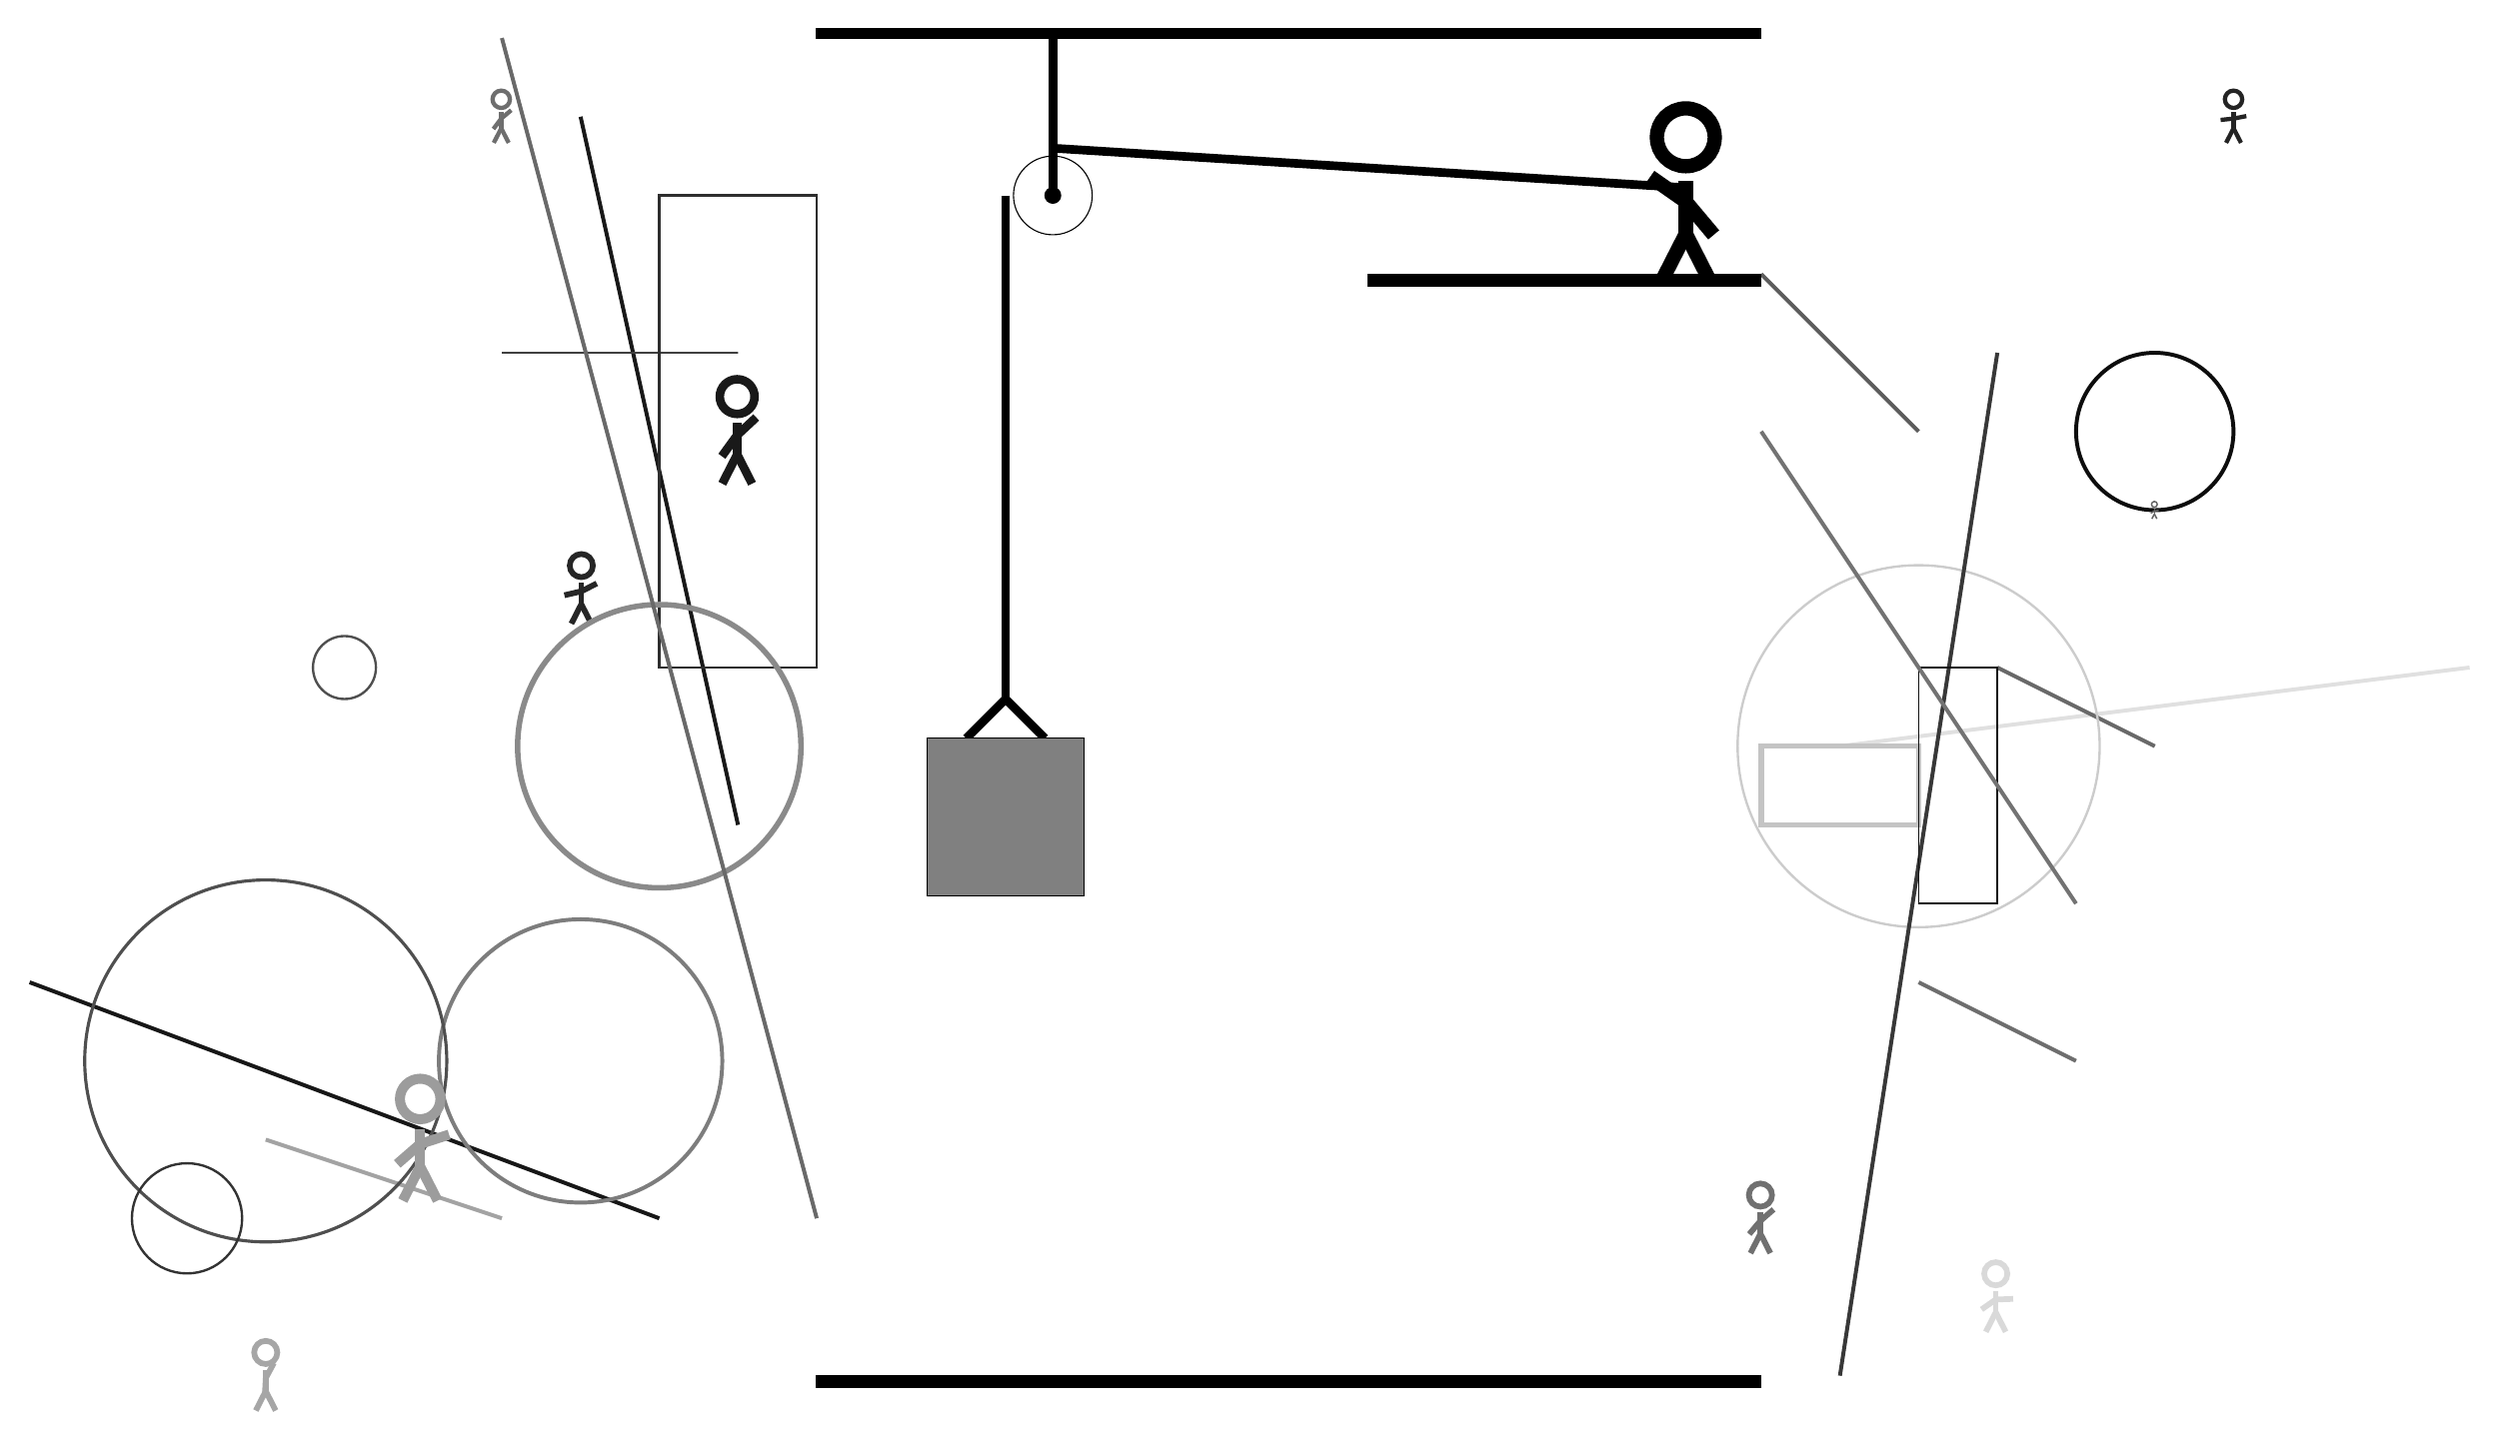
\begin{tikzpicture}
			%%%%% START %%%%%
			
			\draw[fill=black] (-2, 14) rectangle (10, 14.125);
			
			\draw (1, 12) circle (0.5);
			\draw[fill=black] (1, 12) circle (0.1);
			\draw[line width=1.1mm] (1, 14) -- (1, 12);
			
			\draw[line width=0.5mm, color=black!12](11, 5) -- (19, 6);
			
			\draw[line width=0.5mm, color=black!91](-4, -1) -- (-12, 2);
			\draw [line width=0.5mm, color=black!95](15, 9) circle (1.0);
			\draw[line width=0.5mm, color=black!59](13, 6) -- (15, 5);
			\draw [line width=0.3mm, color=black!20](12, 5) circle (2.3);
			\node[line width=0.2mm, color=black!57] at (-6, 13) {\Strichmaxerl[3][53][40]};
			\draw [line width=0.5mm, color=black!51](-5, 1) circle (1.8);
			\node[line width=0.2mm, color=black!90] at (-3, 9) {\Strichmaxerl[6][54][43]};
			\draw[line width=0.5mm, color=black!78](11, -3) -- (13, 10);
			\draw[line width=0.5mm, color=black!90](-3, 4) -- (-5, 13);
			
			\draw[line width=0.3mm, color=black!75] (-3, 10) rectangle (-6, 10);
			
			\draw[line width=0.5mm, color=black!36](-6, -1) -- (-9, 0);
			\draw [line width=0.4mm, color=black!69](-9, 1) circle (2.3);
			
			\draw[line width=0.3mm, color=black!82] (-2, 12) rectangle (-4, 6);
			\draw [line width=0.5mm, color=black!21](12, 8) circle (0.0);
			\node[line width=0.5mm, color=black!85] at (-5, 7) {\Strichmaxerl[4][13][27]};
			
			\draw [line width=0.3mm, color=black!80](-10, -1) circle (0.7);
			
			\node[line width=0.2mm, color=black!86] at (16, 13) {\Strichmaxerl[3][6][11]};
			\draw[line width=0.5mm, color=black!64](10, 11) -- (12, 9);
			\draw [line width=0.3mm, color=black!45](-4, 6) circle (0.0);
			\draw[line width=0.5mm, color=black!57](12, 2) -- (14, 1);
			
			\draw [line width=0.7mm, color=black!46](-4, 5) circle (1.8);
			\draw[line width=0.5mm, color=black!59](-6, 14) -- (-2, -1);
			\draw [line width=0.3mm, color=black!69](-8, 6) circle (0.4);
			\draw[line width=0.7mm, color=black!23] (12, 4) rectangle (10, 5);
			
			\draw[line width=0.2mm, color=black!92] (12, 3) rectangle (13, 6);
			
			\node[line width=0.2mm, color=black!61] at (15, 8) {\Strichmaxerl[1][34][5]};
			\node[line width=0.7mm, color=black!39] at (-7, 0) {\Strichmaxerl[7][41][18]};
			\node[line width=0.7mm, color=black!56] at (10, -1) {\Strichmaxerl[4][50][41]};
			\node[line width=0.2mm, color=black!15] at (13, -2) {\Strichmaxerl[4][35][2]};
			\draw[line width=0.5mm, color=black!55](10, 9) -- (14, 3);
			
			\node[line width=0.5mm, color=black!35] at (-9, -3) {\Strichmaxerl[4][87][62]};
			
			\draw[line width=1.1mm](-0.1, 5.1) --  (0.4, 5.6) -- (0.9, 5.1);
			\draw[fill=black!50] (-0.6, 5.1) rectangle (1.4, 3.1);
			
			\draw[line width=1.1mm](0.4, 12) -- (0.4, 5.6);
			\centerarc[line width=1.1mm](1, 12)(90:180:0.6)
			\draw[line width=1.1mm](1, 12.6) -- (9, 12.1);
			
			\node at (9, 12) {\Strichmaxerl[10][-35][-50]};
			\draw[fill=black] (5, 11) rectangle (10, 10.85);
			
			\draw[fill=black] (-2, -3) rectangle (10, -3.15);
			
			%%%%% END %%%%%
		\end{tikzpicture}
	\end{figure}	
\end{document}